\chapter{Dynamic Transport Services}
\label{ch:dts}
% ##################################################################################################################

\hfill \textbf{Author:} Michal Maciejewski

\begin{center} 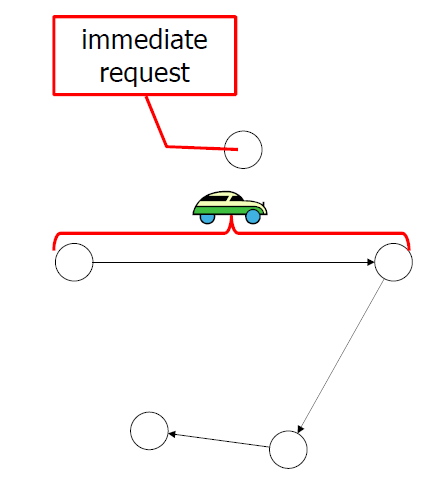
\includegraphics[width=0.4\textwidth, angle=0]{extending/figures/DTS/dts.png} \mm{change this picture} \end{center}

\createStandardInformation{dvrp}{todo}{todo}{todo}

\mm{Alternative title: Dynamic vehicle routing}

% ##################################################################################################################

\section{Introduction}

The recent technological advancements in Information and Communications Technology (ICT), have allowed for emergence of novel on-line fleet management tools and thus opened up a broad range of possibilities for transport services to become more intelligent, that is flexible, demand responsive, safe and energy/cost efficient. This concerns both significant enhancements in operations of the traditional means of transport, such as regular public transport or taxis, as well as the introduction of novel solutions, such as demand-responsive transport or personal rapid transport. However, the growing complexity of modern transport systems, besides all the benefits, increases the risk of poor performance, or even failure, due to the lack of precise design, implementation and testing.

One way of dealing with this problem is to use simulation tools that offer a wide spectrum of possibilities for validating transport service models (e.g.,\,\cite{ReganMahmassaniJaillet1998DynamicFleetManagementSimulation, BarceloEtc2007RoutingSchedulingSimulationLogistics, LiaoEtc2008ObjOrFramework4DVRP} \mm{find better references, incl.\ Agentpolis}).
%
Such tools have to accurately model not only the dynamically changing demand and supply for the service, but also the traffic flow and other existing transport services/modes. To the best knowledge of the author, none of the existing solutions provides large-scale microscopic simulation that is necessary for detailed analysis. 

\mm{Reference to the DVRPs??? Why simulation instead of competitive analysis?}

% ##################################################################################################################

\section{DVRP Extension}

To address the above mentioned problem, MATSim's DVRP ($=$ \emph{Dynamic Vehicle Routing Problem}) extension has been developed. It is meant for simulating a broad scope of dynamic vehicle routing and scheduling processes, and offers additional functionality for simulating passenger on-demand transport services. Typically, the DVRP extension is responsible for modeling both supply and demand, and optimizing fleet operations online, whereas the MATSim's core is used for simulating supply and demand, both embedded into a large-scale microscopic transport simulation. In particular, it is assumed that:
%
\begin{itemize}
	\item each driver is modeled as an agent that follows his/her dynamic schedule; this is in contrast to the standard day-to-day learning approach used in MATSim

	\item a driver’s/vehicle’s schedule is a sequence of tasks of different types, such as driving from one location to another or waiting at a given location

	\item optimization is triggered by events that reflect changes in the system

	\item a fleet of vehicles comprises one component of the whole traffic flow simulated by means of one of the queue-based simulators available in MATSim

	\item each vehicle can be monitored online as it moves from link to link; this information may be used to update the timing of its schedule and possibly trigger re-optimization

	\item in the case of passenger transport (e.g. taxi, DRT), interaction between the dispatcher, drivers and pas-sengers is simulated in detail, including calling a ride, picking up/dropping off passengers, etc.
\end{itemize}


%In particular, the extension is responsible for:
%%
%\begin{itemize}
	%\item modeling the DVRP domain
	%\item listening to simulation events
	%\item monitoring the state of simulation (e.g.\ movement of vehicles)
	%\item finding least-cost paths
	%\item computing schedules for drivers/vehicles
	%\item binding drivers' behavior to their schedules
	%\item coordinating interaction/cooperation between drivers, passengers and dispatchers (e.g.\ handling requests submissions, letting people in and out of vehicles)
%\end{itemize}

The DVRP extension is intended to be as general and customizable as possible. Currently, the domain model is capable of representing a wide range of one-to-many and many-to-many VRPs, and one can easily extend the model even further to cover other specific cases. Since the central focus is on the dynamic optimization algorithm, the architecture of the DVRP extension allows plugging in various algorithms. At present, there are several different algorithms available, among them a memetic algorithm for the \emph{Dynamic Multi-Depot Vehicle Routing Problem with Time Windows and Time-Dependent Travel Times and Costs} analyzed in \citep{MaciejewskiNagel2011DVRPMatsim}, and a family of algorithms for online taxi dispatching discussed in \mm{.........}.

Dynamic transport services, such as taxi services, are simulated in MATSim as one of the components of a transport system. The optimizer plugged into the DVRP extension reacts to selected events generated during simulation. Those events can be request submissions, vehicle departures or arrivals, etc. Additionally, it can monitor the movement of individual vehicles, as well as query other sources of online information, for instance, about the current traffic conditions. In response to the changes in the system, the optimizer may update drivers' schedules, either by applying smaller modifications or re-optimizing them from scratch. Drivers are notified about changes in their schedules and adjust to them as soon as possible; in the most extreme approach vehicles may be even immediately diverted from their current destinations.

% ##################################################################################################################

\section{DynAgent}
\label{sec:dynAgent}
\mm{move after Section DVRP model?}

Contrary to the standard day-to-day learning in MATSim, in the DVRP extension, each driver is behaves dynamically and follows the orders continuously coming from the dispatcher. The \lstinline$DynAgent$ class, along with the \lstinline$org.matsim.contrib.dynagent$ package, provides the foundation for simulating such dynamically behaving agents. Although  being created for the needs of the DVRP extension, \lstinline$DynAgent$ is not limited to this context only, and can be applied in a wide range of different simulation scenarios where dynamism of agents is required.

The main idea behind \lstinline$DynAgent$ is that instead of using a pre-computed (and occasionally re-computed; see \ref{sec:impl-plan-based}) plan, an agent can actively decide what to do at each simulation step. It is up to the agent, whether decisions are made on the fly or (re-)planned in advance. In some applications, a \lstinline$DynAgent$ may represent a fully autonomous agent that acts according to his/her desires, beliefs and intentions, whereas in other cases, it may a non-autonomous agent following orders that are systematically coming from the outside (e.g. a driver receiving tasks from a centralized vehicle dispatching system).

\subsection{Main interfaces and classes}

The \lstinline$DynAgent$ class is a dynamic implementation of \lstinline$MobsimDriverPassengerAgent$. Instead of executing pre-planned \lstinline$Activity$s and \lstinline$Leg$s, a \lstinline$DynAgent$ performs \lstinline$DynActivity$s and \lstinline$DynLeg$s. The following assumptions underlie the agent's behavior:
%
\begin{itemize}
	\item the \lstinline$DynAgent$ is the physical representation of the agent, responsible for the interaction with the real world (i.e., traffic simulation)

	\item the agent's high-level behavior is controlled by a \lstinline$DynAgentLogic$ that can be seen as the agent's brain; the \lstinline$DynAgentLogic$ is responsible for deciding on the agent's next action (leg or activity) once the current one has ended
	
	\item dynamic legs and activities fully define the agent's low-level behavior, down to the level of a single step in simulation.
\end{itemize}
%
At the higher level, the dynamism of the \lstinline$DynAgent$ results from the fact that dynamic activities and legs are usually created on the fly by the agent's \lstinline$DynAgentLogic$, thus the agent does not have to plan future actions in advance. In the case when the agent has a more or less detailed plan of legs and activities, the agent does not have to adhere to it, and may modify his/her plan at any time (e.g., change the mode or destination of a future leg, or include or omit a future activity).

The low-level dynamism is provided by the mechanism of executing dynamic activities and legs. As for the currently executed activity, the agent can shorten or lengthen its duration at any time. Additionally, at each time step, the agent may decide upon what to do right now (e.g., communicate with other agents, re-plan the next activity or leg, and so on). In the case of driving a car (\lstinline$DriverDynLeg$), the agent can change the route, destination or even decide upon picking up or dropping off somebody on the way. When using the public transport (\lstinline$PTPassengerDynLeg$), the agent chooses which bus to get on and which stop to exit at.

Incidentally, the behavior of MATSim's default plan-based agent, \lstinline$PersonDriverAgentImpl$, can be simulated by \lstinline$DynAgent$ combined with the \lstinline$PlanToDynAgentLogicAdapter$ logic. This adapter class creates series of dynamic activities and legs that mimics a given \lstinline$Plan$ of static \lstinline$Activity$s and \lstinline$Leg$s.

\subsection{Configuring and running a dynamic simulation}
\label{sec:config-dyn-sim}

\lstinline$DynAgent$ has been written for and validated aginst \lstinline$QSim$. Simulation of dynamic legs does not require any additional code. However, to take advantage of dynamic activities,  \lstinline$DynActivityEngine$ should be used instead of \lstinline$ActivityEngine$. \lstinline$DynActivityEngine$'s \lstinline$doSimStep(double time)$ method ensures that dynamic activities are actively executed by agents and their end times can be changed.

The easiest way to run a single iteration of \lstinline$QSim$ is as follows:
%
\begin{enumerate}

	\item Call \lstinline$DynAgentLauncherUtils$' \lstinline$initQSim(Scenario scenario)$ method to create and initialize a \lstinline$QSim$; this includes creating a series of objects, such as an \lstinline$EventsManager$, \lstinline$DynActivityEngine$, or \lstinline$TeleportationEngine$

	\item Add \lstinline$AgentSource$s of \lstinline$DynAgent$s and other agents to the \lstinline$QSim$
	
	\item Run simulation by calling \lstinline$QSim$'s \lstinline$run()$ method
	
	\item Finalize processing events by calling \lstinline$EventsManager$'s \lstinline$finishProcessing()$ method
	
\end{enumerate}
%
Depending on the needs, the above procedure can be extended with additional steps, such as adding non-default engines or departure handlers to the \lstinline$QSim$.

\subsection{RandomDynAgent Example}
\mm{combine this section with previous}

The \lstinline$org.matsim.contrib.dynagent.examples.random$ package contains a basic illustration of how to create and run a scenario with \lstinline$DynAgent$s. To highlight the contrast to the plan-based agents, in this example, 100 dynamic agents travel randomly (\lstinline$RandomDynLeg$) and perform activities of random duration (\lstinline$RandomDynActivity$).

The high-level random behavior is controlled by \lstinline$RandomDynAgentLogic$ that operates according to the following rules:
%
\begin{enumerate}

	\item Each agent starts with a \lstinline$RandomDynActivity$; see the \lstinline$computeInitialActivity(DynAgent agent)$ method
	
	\item Whenever the currently performed activity or leg ends, a random choice on what to do next is made between the following options: (a) stop being simulated by starting a deterministic \lstinline$StaticDynActivity$ with infinite end time, (b) start a \lstinline$RandomDynActivity$, or (c) start a \lstinline$RandomDynLeg$; see the \lstinline$computeNextAction(DynAction oldAction, double now)$ method

\end{enumerate}

The stochasticity at the lower level results from random decisions being made at each consecutive decision point. In the case of \lstinline$RandomDynLeg$, each time an agent enters a new link, he or she decides whether to stop at this link or to continue driving; in the latter case, the subsequent link is chosen randomly; see the \lstinline$RandomDynLeg(Id<Link> fromLinkId, Network network)$ constructor and the \lstinline$movedOverNode(Id<Link> newLinkId)$ method. As for \lstinline$RandomDynActivity$, at each time step, the \lstinline$doSimStep(double now)$ method is called and a random decision is made on the activity end time.

Following the rules specified in Section~\ref{sec:config-dyn-sim}, setting up and running this example scenario is straightforward. \lstinline$RandomDynAgentLauncher$ reads a network, initializes a \lstinline$QSim$, then adds a \lstinline$RandomDynAgnetSource$ to the \lstinline$QSim$, and finally, launches visualization and starts simulation. The \lstinline$RandomDynAgentSource$ is responsible for instantiating 100 \lstinline$DynAgent$s that are randomly distributed over the network. The simulation ends when the last active agent becomes inactive.

% ##################################################################################################################

\section{VRP model}

The DVRP extension can be used for rich vehicle routing problems. The major extensions in the VRP model, compared to the classical and very popular Capacitated VRP, are as follows:
%
\begin{itemize}
	\item one-to-many (many-to-one) and many-to-many topologies
	\item multiple depots
	\item dynamic requests
	\item request and vehicle types
	\item time windows for requests and vehicles
	\item time-dependent stochastic travel times
	\item time-dependent stochastic travel costs
	\item network-based routing (including vehicle monitoring and diversion)
\end{itemize}
%
Except for the travel times and costs (discussed in Section~\ref{sec:VRP-router}), which are calculated on demand, all the VRP-related data are stored in or accessible via \lstinline$VrpData$%
\footnote{
Package \lstinline$org.matsim.contrib.dvrp.data$.
}.
In the most basic setup, there are only two types entities, namely \lstinline$Vehicle$s and \lstinline$Request$s, whereas for managing a fleet of electric vehicles, for instance, a specialized data container, \lstinline$ElectricVrpData$, stores information about \lstinline$Charger$s%
\footnote{
Package \lstinline$org.matsim.contrib.dvrp.extensions.electric$.
}.
Another implemented extension of the model supports pickups and deliveries (the \emph{Vehicle Routing Problem with Pickup and Delivery}\mm{add ref??})%
\footnote{
Package \lstinline$org.matsim.contrib.dvrp.extensions.vrppd$.
}.

\subsection{Schedule}
\label{sec:VRP-schedule}

Each \lstinline$Vehicle$ has a \lstinline$Schedule$ that is a sequence of \lstinline$Task$s of different types, such as driving from one location to another (\lstinline$DriveTask$), or staying (e.g., serving a customer or waiting) at a given location (\lstinline$StayTask)$%
\footnote{
Package \lstinline$org.matsim.contrib.dvrp.schedule$.
}. \lstinline$Schedule$ is the point where supply and demand meet each other. All schedules are calculated by an online optimization algorithm (see Section~\ref{sec:VRP-optimizer}) that represents the fleet's dispatcher. Each task is in one of the following states (defined in the \lstinline$Task.TaskStatus$ enum): \lstinline$PLANNED$, \lstinline$STARTED$, \lstinline$PERFORMED$ or \lstinline$CANCELLED$, whereas each schedule is in one of the following states:
%
\begin{itemize}
	\item \lstinline$UNPLANNED$ -- no tasks assigned
	
	\item \lstinline$PLANNED$ -- all tasks are \lstinline$PLANNED$ (none of them has been started)
	
	\item \lstinline$STARTED$ -- one of the tasks is \lstinline$STARTED$ (this is the schedule's \lstinline$currentTask$; the preceding tasks are \lstinline$PERFORMED$ and succeeding tasks are \lstinline$PLANNED$)
	
	\item \lstinline$COMPLETED$ -- all tasks are \lstinline$PERFORMED$
\end{itemize}
%
In general, when modifying a \lstinline$Schedule$, one can change and rearrange the planned tasks, whereas the performed ones are considered to be read-only. In the case of the current task, one can, for instance, change its end time, while the start time remain cannot be changed. Proceeding to the next task may be carried out either by finishing the current one (\lstinline$Schedule.nextTask()$) or canceling it (\lstinline$Schedule.cancelTaskAndNextTask()$).

The execution of the current task may be monitored by means of \lstinline$TaskTracker$%
\footnote{
Package \lstinline$org.matsim.contrib.dvrp.tracker$.
}.
In the most basic version, a tracker only predicts the end time of the current task. More complex trackers give also detailed information on the current state of the task execution. \lstinline$OnlineDriveTaskTracker$, for example, offers functionality similar to that of GPS navigation, such as monitoring the movement of a vehicle, predicting its arrival time and even diverting its path.

\lstinline$ScheduleImpl$, along with \lstinline$DriveTaskImpl$ and \lstinline$StayTaskImpl$, is the default implementation of \lstinline$Schedule$ and offers several additional features, such as data validation or automation of handling tasks. It also serves as the starting point when implementing domain-specific schedules or tasks (e.g. \lstinline$ChargeTask$ in the electric VRP model mentioned above).

\subsection{Least-cost paths}
\label{sec:VRP-router}

MATSim's network model consists of nodes connected by one-way links. Because of the queue-based traffic flow simulation (Section~\ref{sec:trafficflowmodel}), a link is the smallest traversable element. Besides links, the DVRP extension operates also on a higher level of abstraction, that is paths. Each path is a sequence of links to be traversed to get from one location to another in the network, or more precisely, from the end of one link end to the end of another link. 

The functionality of finding least-cost paths is implemented in the \lstinline$org.matsim.contrib.dvrp.router$ package. \lstinline$VrpPathCalculator$ calculates \lstinline$VrpPath$s by means of the least-cost path search algorithms available in Matsim's core%
\footnote{
Package \lstinline$org.matsim.core.router$.
}
\citep{JacobMaratheEtAl1999computationalstudyof,LefebvreBalmer2007Fastshortestpath}. Because of changeable traffic conditions, paths are calculated for a given departure time. Since MATSim calculates averaged travel time statistics for links for every 15-minute time period by default, the 15-minute time bin is also used for computing shortest paths.

\lstinline$VrpPath$s are used by \lstinline$DriveTask$s to specify the sequence of links to be traversed by a vehicle between two locations. It is possible to divert a vehicle from its destination by replacing the currently followed \lstinline$VrpPath$ with a \lstinline$DivertedVrpPath$.

To reduce computational burden, the already calculated paths can be cached for future reuse (see \lstinline$VrpPathCalculatorWithCache$). However, when calculating least-cost paths from one location to many potential destinations, a significant speed-up can be achieved by means of least-cost tree search (see \lstinline$org.matsim.utils.LeastCostPathTree$).

% ##################################################################################################################

\section{Agents}

Realistic simulation of dynamic transport services requires proper representation of interaction and possible collaboration between the main actors, that is drivers, customers (often being passengers), and a dispatcher. By default, drivers and passengers are simulated as agents whereas dispatcher's operations are modeled as an optimization algorithm (see Section~\ref{sec:VRP-optimizer}). This, however, does not exclude other configurations (e.g., a decentralized system without a dispatcher).

\subsection{Drivers}
\label{sec:VRP-agent}

A driver is modeled as a \lstinline$DynAgent$ whose behavior is controlled by a \lstinline$VrpAgentLogic$%
\footnote{
Package \lstinline$org.matsim.contrib.dvrp.vrpagent$.
}
that makes the agent follow the dynamically changing \lstinline$Schedule$. As a result, all changes made to the schedule are visible to and obeyed by the driver. Whenever a new task is started, the driver logic converts it to the corresponding dynamic action. Specifically, a \lstinline$DriveTask$ is executed as a \lstinline$VrpLeg$, whereas a \lstinline$StayTask$ is simulated as a \lstinline$VrpActivity$. Both \lstinline$VrpLeg$ and \lstinline$VrpActivity$ are implemented in such a way that any change to the referenced task is automatically visible to them. At the same time, any progress made while carrying them out, is instantly reported to the referenced task's tracker.

\subsection{Passengers}
\label{sec:VRP-passengers}

A special type of customers are passengers in dynamic transport services. In order to simulate their trips microscopically, passengers are modeled as \lstinline$MobsimPassengerAgent$s. Being a part of the simulation, they can board, ride and finally exit vehicles. In contrast to the drivers, they may be modeled as the standard MATSim agents, each of them having a fixed daily plan consisting of legs and activities.

The interaction between drivers, passengers and the dispatcher, which includes a sequence of submitting a \lstinline$PassengerRequest$ and then picking up and dropping off the passenger, is coordinated by a \lstinline{PassengerEngine}%
\footnote{
Package \lstinline$org.matsim.contrib.dvrp.passenger$.
}.
Requests may be immediate (\emph{as soon as possible}) or advance (\emph{at the appointed time}). In the former case, a passenger starts waiting just after placing the order, whereas in the latter case, the dispatched vehicle my arrive at the pickup location before or after the designated time, which means that either the driver or the customer, respectively, will wait for the other to come. To ensure the proper coordination between these two agents, the pickup activity performed by the driver must implement the \lstinline$PassengerPickupActivity$ interface.

% ##################################################################################################################

\section{Optimizer}
\label{sec:VRP-optimizer}

Since demand and supply are inherently stochastic, the general approach to dealing with dynamic transport services consists in updating vehicles' schedules in response to observed changes (modeled as events). This can be done by means of re-optimization procedures that consider all the requests (within a given time horizon) or fast heuristics focused on small updates of the existing solution rather than constructing a new one from scratch. Usually, re-optimization procedures give solutions of higher quality compared to the local update heuristics, however, when it comes to the real-world applications, where high (often real-time) responsiveness is crucial, broad re-optimization may be prohibitively time consuming.

In the most basic case, an optimizer implements the \lstinline$VrpOptimizer$ interface%
\footnote{
Package \lstinline$org.matsim.contrib.dvrp.optimizer$.
},
that is, implements the following two methods:
%
\begin{itemize}
	\item \lstinline$requestSubmitted(Request request)$ -- called on submitting \lstinline$request$; in response, the optimizer either adapts vehicles' schedules so that \lstinline$request$ can be served, or rejects the order
	
	\item \lstinline$nextTask(Schedule<? extends Task> schedule)$ -- called whenever \lstinline$schedule$'s current task has been completed and the driver is switching to the next planned task; this is the last moment to make the final decision upon what to do next;

\end{itemize}

This basic functionality can be easily extended. Besides request submission, one may, for example, consider modifying or even canceling already submitted requests. Another option is monitoring vehicles as they travel along designated routes and reacting when they are ahead of/behind their schedules. Such functionality is available by implementing \lstinline$VrpOptimizerWithOnlineTracking$'s \lstinline$nextLinkEntered(DriveTask driveTask)$ method, which is called whenever a vehicle moves from the current link to the next one on its path.

Last but not least, there are two ways of responding to the incoming events. They can be handled either \emph{immediately} (\emph{synchronously}) or \emph{between time steps} (\emph{asynchronously}). In the former case, schedules are re-calculated (update, re-optimized) directly in response to calling one of the optimizer's methods. This simplifies accepting/rejecting new requests since the answer is immediately passed back to the caller. In the latter case, all events within a simulation step are recorded and then processed in batch mode just before the next simulation step begins. By doing that one can not only reduce significantly the computational demand, but also avoid situations when due to vehicles' inertia (e.g., activities may end only at the beginning of the simulation step), two or more mutually conflicting decisions could be made.

% ##################################################################################################################

\section{Configuring and running a DVRP simulation}

Like in within-day replanning (see Section~\ref{ch:withinday}), dynamic transport services are typically run with the DVRP extension as a single-iteration simulation.

\mm{combine this section and OneTaxi example}

\begin{itemize}
	\item Initialize a \lstinline$Scenario$ that holds MATSim's domain data (see: \lstinline$VrpLauncherUtils.initScenario$ methods)
	
	\item Create a \lstinline$$initVrpData that holds VRP's domain data (see: \lstinline$VrpLauncherUtils.initVrpData$)
	
	\lstinline$MatsimVrpContext$ object that holds references to a \lstinline$VrpData$ (VRP's domain data), \lstinline$Scenario$ (MATSim's domain data) and \lstinline$MobsimTimer$ (\lstinline$QSim$'s timer)
	
	\item Create a \lstinline$VrpData$ to store all VRP-based data 
	
	\item Create a \lstinline$VrpPathCalculator$ or other router, such as \lstinline$LeastCostPathTree$, 
	
	\item Instantiate \lstinline$VrpOptimizer$
	
	\item \lstinline$QSim$
	
	\item \lstinline$PassengerEngine$
	
	\item \lstinline$DynActionCreator$
	
	\item \lstinline$EventsManager$
	
\end{itemize}

% ##################################################################################################################

\section{OneTaxi example}

There are ten taxi customers and one taxi driver, who serves all requests in the FIFO order. Each customer dials a taxi at some time to get from work to home. The example is made up of 6 quite simple classes:
%
\begin{itemize}
	\item \lstinline$OneTaxiRequest$ -- represents taxi requests
	
	\item \lstinline$OneTaxiRequestCreator$ -- converts taxi calls into requests that are submitted to the optimizer
	
	\item \lstinline$OneTaxiOptimizer$ -- builds/updates the taxi driver's schedule
	
	\item \lstinline$OneTaxiServeTask$ -- represents stay tasks related to serving customers (i.e. picking up and dropping off)
	
	\item \lstinline$OneTaxiActionCreator$ -- converts schedule elements (tasks) into dynamic actions (i.e. dynamic activities or legs)
	
	\item \lstinline$OneTaxiLauncher$ -- sets up and runs the whole scenario
\end{itemize}

The example is located in the \lstinline$org.matsim.contrib.dvrp.examples.onetaxi$ package. All data is stored in the \lstinline$/contrib/dvrp/src/main/resources/one_taxi$ directory.







\mm{assesing the performance}
Either by analysing Schedules: playground.michalm.taxi.optimizer.TaxiStatsCalculator, or listening to events: playground.jbischoff.taxi.evaluation.TravelDistanceTimeEvaluator or playground.jbischoff.taxi.evaluation.TaxiCustomerWaitTimeAnalyser 
Both ways should give same results.

Subclassing/extending Requests and Tasks is helpful (e.g. OneTaxiServeTask).

% ##################################################################################################################

\section{Research with DVRP/Conclusions}

this will be a kind of conclusions. Past, ongoing and possible future projects based on DVRP. Possible future developments/enhancements of DVRP.

\mm{Add papers from Nicole (mail on 25/08/2014 08:48)}
\mm{Cross-reference from Nicole's and my scenarios to DVRP}

% ##################################################################################################################
%Joschka Bischoff as author?
%Taxis Berlin: electric vehicles -> pres Wiepersdorf
%
%Mielec and Berlin Scenarios
%
%http://www.matsim.org/node/379
%
%\kwaah{does MATSim 2030 help here?}

% ##################################################################################################################
